\newpage
\appendix
	\begin{table}[h]
		\[
		\begin{split}
			&0 \rightarrow 1 \rightarrow 2 \rightarrow 3 \rightarrow 0 \quad \text{dist}=28 \hspace{1cm} 1 \rightarrow 0 \rightarrow 2 \rightarrow 3 \rightarrow 1 \quad \text{dist}=18 \\
			&0 \rightarrow 1 \rightarrow 3 \rightarrow 2 \rightarrow 0 \quad \text{dist}=18 \hspace{1cm} 1 \rightarrow 0 \rightarrow 3 \rightarrow 2 \rightarrow 1 \quad \text{dist}=28\\
			&0 \rightarrow 2 \rightarrow 1 \rightarrow 3 \rightarrow 0 \quad \text{dist}=20 \hspace{1cm} 1 \rightarrow 2 \rightarrow 0 \rightarrow 3 \rightarrow 1 \quad \text{dist}=20\\
			&0 \rightarrow 2 \rightarrow 3 \rightarrow 1 \rightarrow 0 \quad \text{dist}=18 \hspace{1cm} 1 \rightarrow 2 \rightarrow 3 \rightarrow 0 \rightarrow 1 \quad \text{dist}=28\\
			&0 \rightarrow 3 \rightarrow 1 \rightarrow 2 \rightarrow 0 \quad \text{dist}=20 \hspace{1cm} 1 \rightarrow 3 \rightarrow 0 \rightarrow 2 \rightarrow 1 \quad \text{dist}=20\\
			&0 \rightarrow 3 \rightarrow 2 \rightarrow 1 \rightarrow 0 \quad \text{dist}=28 \hspace{1cm} 1 \rightarrow 3 \rightarrow 2 \rightarrow 0 \rightarrow 1 \quad \text{dist}=18\\ \\
			%
			&2 \rightarrow 0 \rightarrow 1 \rightarrow 3 \rightarrow 2 \quad \text{dist}=18 \hspace{1cm} 3 \rightarrow 0 \rightarrow 1 \rightarrow 2 \rightarrow 3 \quad \text{dist}=28 \\
			&2 \rightarrow 0 \rightarrow 3 \rightarrow 1 \rightarrow 2 \quad \text{dist}=20 \hspace{1cm} 3 \rightarrow 0 \rightarrow 2 \rightarrow 1 \rightarrow 3 \quad \text{dist}=20\\
			&2 \rightarrow 1 \rightarrow 0 \rightarrow 3 \rightarrow 2 \quad \text{dist}=28 \hspace{1cm} 3 \rightarrow 1 \rightarrow 0 \rightarrow 2 \rightarrow 3 \quad \text{dist}=18\\
			&2 \rightarrow 1 \rightarrow 3 \rightarrow 0 \rightarrow 2 \quad \text{dist}=20 \hspace{1cm} 3 \rightarrow 1 \rightarrow 2 \rightarrow 0 \rightarrow 3 \quad \text{dist}=20\\
			&2 \rightarrow 3 \rightarrow 0 \rightarrow 1 \rightarrow 2 \quad \text{dist}=28 \hspace{1cm} 3 \rightarrow 2 \rightarrow 0 \rightarrow 1 \rightarrow 3 \quad \text{dist}=18\\
			&2 \rightarrow 3 \rightarrow 1 \rightarrow 0 \rightarrow 2 \quad \text{dist}=18 \hspace{1cm} 3 \rightarrow 2 \rightarrow 1 \rightarrow 0 \rightarrow 3 \quad \text{dist}=28\\
		\end{split}
		\]
		\caption{Solutions to TSP in Figure \ref{fig:tsp}. Each eigenvector forms a tour about the graph with an associated eigenvalue corresponding to the total distance traveled. The optimal ground state eigenvalue 18 corresponds to a set of possible eigenvectors.}
		\label{tab:eigenset}
	\end{table}
	\begin{center}
		\begin{figure}[h]
			\begin{center}
				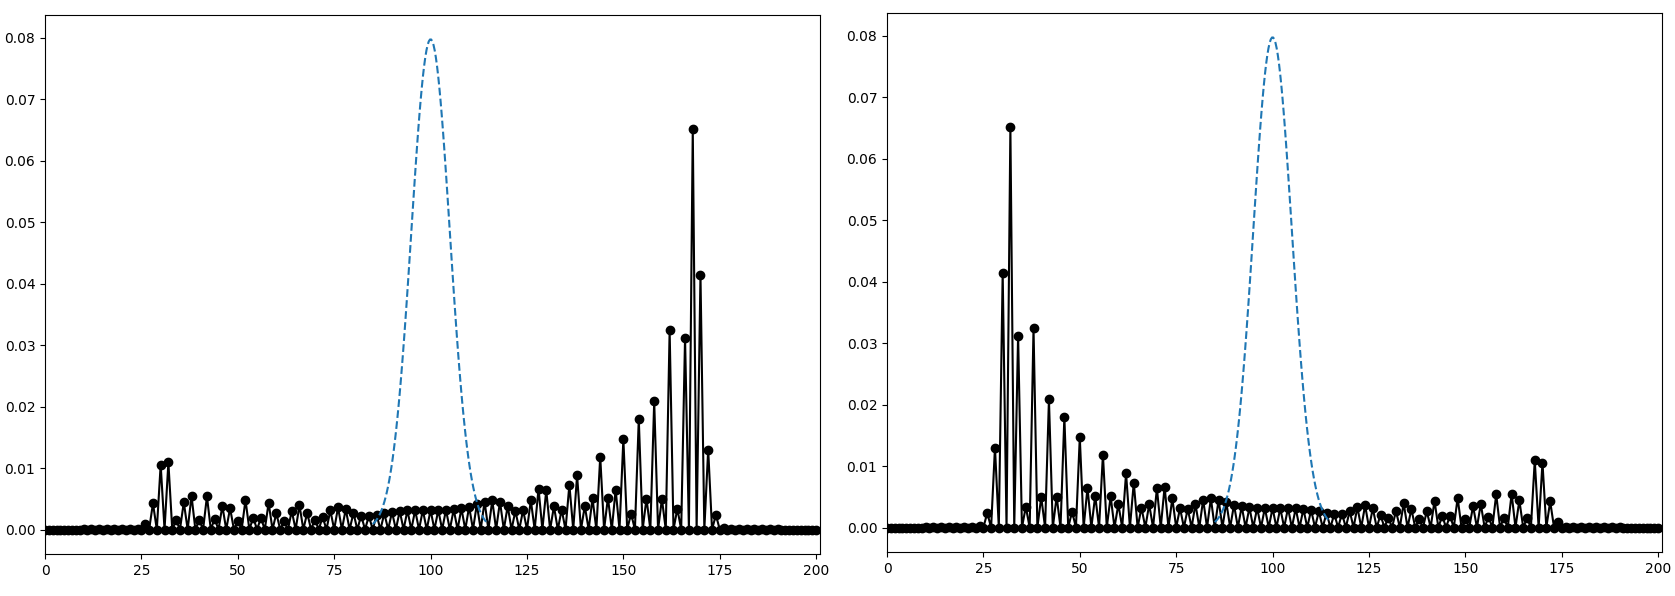
\includegraphics[width=16cm]{images/bias}
			\end{center}
			\caption{Plot of the probability distributions of a classical random walk an a quantum random walk. The blue dotted line in each plot is the result of a classical Gaussian distribution. In the left plot, the black distribution is the result of preparing the quantum walk with a particle in a pure spin-up configuration $|\Psi\rangle = |0\rangle$. In the right plot, the particle is prepared in a spin-down configuration $|\Psi\rangle = |1\rangle$. In both cases, the quantum distribution exhibits de-constructive interference about the origin, however it is possible to impose a bias toward a particular direction simply by initializaing the system with different weights in $\alpha$ and $\beta$ from Equation \ref{eq:spinStates}.}
			\label{fig:biasWalk}
		\end{figure}
	\end{center}
